\chapter{A1}

{\LARGE 'Compute the total number of packets and bytes (in and out) per protocol (TCP, UDP, ICMP, …) contained in the flows.'}

\section{Explicação do código desenvolvido}

A computação deste tópico foi relativamente fácil, onde apenas foi necessário iterar todos os tuplos do ficheiro, verificar o seu protocolo e adicionar a uma mapa o eu número de \textit{bytes} e \textit{packets}. Como já foi referido, neste tópico utilizamos uma estrutura de dados \textit{(Key, Value)} para guardar em memória os resultados de cada iteração. O código seguinte mostra a parte do \textit{script} que trata de cada tuplo do ficheiro.

\begin{figure}[h]
    \label{high}
    \centering
    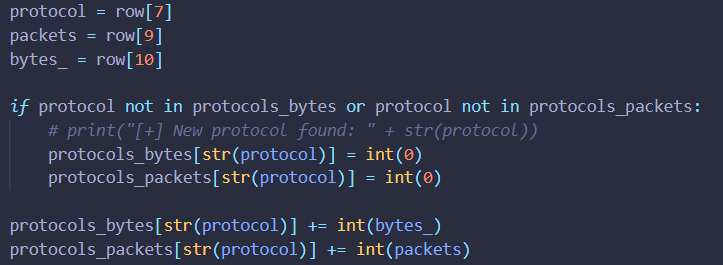
\includegraphics[width=1\textwidth]{Images/a1/a1.png}
    \caption{\textit{Código do tópico a1}}
\end{figure}

%----------------------------------------------------------------------------
%----------------------------------------------------------------------------

\clearpage

\section{Resulados obtidos pelo ficheiro www.fct.unl.pt.csv}

Como se pode ver na figura 2.2, foram processadas as 21362 linhas do ficheiro www.fct.unl.pt.csv, existindo fluxos TCP, UDP e ICMP, estando associados a cada um destes o número de \textit{bytes} e \textit{packets} como pretendido.

\begin{figure}[h]
    \label{high}
    \centering
    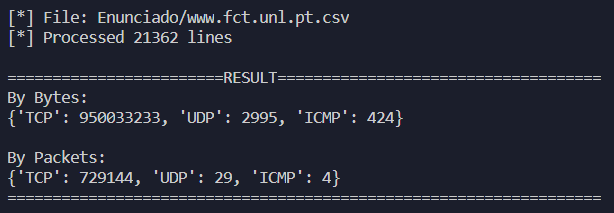
\includegraphics[width=1\textwidth]{Images/a1/a1_a.png}
    \caption{\textit{Output do script a1.py}}
\end{figure}

%----------------------------------------------------------------------------

\section{Resulados obtidos pelo ficheiro bigFlows.csv}

Na figura 2.3 verificamos a mesma estrutura de resultados mas agora para o ficheiro bigFlows.csv, onde podemos verificar que este apresenta um tipo de protocolo que não existia no ficheiro anterior, IGMP.

\begin{figure}[h]
    \label{high}
    \centering
    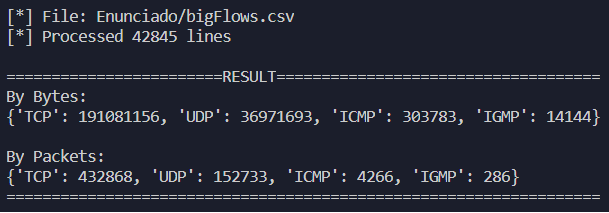
\includegraphics[width=1\textwidth]{Images/a1/a1_b.png}
    \caption{\textit{Output do script a1.py}}
\end{figure}